APE has been used to synthesize and explore scientific workflows in numerous use cases, such as geovisualization and question answering \cite{kasalica2022synthesis}. However, applying the framework and its concepts to the field of data science presents a novel set of challenges, some of which were already briefly mentioned while modeling the ontology in \autoref{ch:ds_ontoloty}. This chapter delves into the details of extending the APE workflow and adapting the data science ontology to achieve the set target of executable Jupyter notebooks.

First, we will examine the difficulties of combining the domain and tabular-data-specific requirements with APE’s synthesis concept to construct workflows with lower-level tools that will run in a general-purpose programming framework. These include the higher-than-usual dimension and input count, the direct management of data references by the user, and the data flow handling by tools in APE’s encoding.

Next, we will revisit the data science ontology, focusing on the modifications for a final version compatible with native APE. The section will give a short rundown of the new tools and slimmed-down type taxonomy while offering insight into the rationale behind these changes.

Finally, we will discuss the implementation details of how the APE workflow was adapted to fit the data science domain better. Here, we introduce a new input data preparation tool, the APE output parser, and the library of wrapped Python tools that facilitate the automated creation of executable Jupyter notebooks.

\section{Challenges}\label{sec:native_ape_challenges}
Combining APE with the data science ontology and use cases defined in \autoref{ch:ds_ontoloty} with no adaptations leads to numerous challenges regarding SAT search, workflow executability, and user interactions. The reason for this lies in the SAT encoding of the workflow search, which, as will be shown, is unsuitable for working with tabular data in some aspects. This section will overview the most prominent issues and discuss potential workarounds where possible.

\subsection{Workflow Encoding}
To gain a basic understanding of the ontology-based synthesis process, we will examine the workflow formula of the SAT encoding in \autoref{eqn:workflow_sat_enc}:
\begin{align}
    \label{eqn:workflow_sat_enc}
    \llbracket W \rrbracket_n := & \bigwedge_{i=1}^{n}\left(\bigvee_{op\in L^\circ} op(m_i)\right)\\
    & \bigwedge_{i=0}^{n}\bigwedge_{j=0}^{k-1}\left(\bigvee_{ty\in L^t} ty(in_i^j)\right)\nonumber\\
    & \bigwedge_{i=0}^{n-1}\bigwedge_{j=0}^{l-1}\left(\bigvee_{ty\in L^t} ty(out_i^j)\right)\nonumber\\
    & \bigwedge_{i=0}^{n-1}\bigwedge_{j=0}^{k-1}\left(\epsilon(in_i^j)\vee\bigvee_{p=0}^{i-1}\bigvee_{q=0}^{l-1}Bind(in_i^j, out_p^q)\right)\nonumber
\end{align}
APE encodes a workflow $[[W]]_n$ as a sequence of \(n\) steps, each having a set of inputs and outputs. Within this encoding:
\begin{itemize}
    \item Each step \(i\) uses a tool \(op\) from the ontology. An auxiliary encoding enforces the tool and type taxonomy properties, such that using a non-leaf node implicates the usage of one of its child nodes and vice-versa.
    \item Input and output parameters are so-called type states \(ty\), defined by their type dimensions. APE uses the same number of parameters with every tool and adds empty type states \(\epsilon\) for tools with fewer.
    \item Any non-empty input type state can be bound to an output type state of a previous tool, ensuring the dependencies in the linear sequence. To add external IO, workflow inputs and outputs are added as the \(0\)th tool's outputs and the \(n+1\)th tool's inputs.
\end{itemize}

\subsection{Input Labels}\label{sec:input_labels}
Since type states derive their values from the dimensions defined in the ontology, a tool parameter can only adopt values already defined in the type taxonomy. Hence, it is impossible to use constraints to introduce arbitrary inputs to the workflow, such as new column labels or numerical graph sizes. As a result, selected values must be added to both the taxonomy and workflow inputs before the user can utilize them in constraints. This can be done without changing the ontology by using \verb|APE_label|, an implicit type dimension created by APE during runtime with an empty default label. Any values in the workflow input listed under that dimension, as illustrated in \autoref{code:APE_label_IO}, are appended to the sub-taxonomy and can then be referenced during the synthesis process and the workflow execution.

\begin{lstlisting}[language=json, caption=Example of APE IO Configuration., label=code:APE_label_IO]
"inputs": [
  {
    "DataClass": ["StrColumn"],
    "APE_label": ["Name"]
  },
  {
    "DataClass": ["Int"],
    "APE_label": ["42"]
  }
],
"outputs": [
  {
    "DataClass": ["Figure"]
  }
]
\end{lstlisting}

However, because APE adds these labels during its runtime, none appear in any tool transition rule. Consequently, no tool produces labeled outputs, and type states with an explicit \verb|APE_label| value only exist as workflow inputs. Modifying the tool annotations to account for this new dimension with potentially as many values as inputs would increase the search complexity by a drastic amount, as shown later in this section.

\subsection{APE Data Flow}
Moreover, the \(bind\) predicate may assign any already generated outputs to a tool input, even if they have already been used earlier. Instead of message passing, this memory bus architecture leaves inputs available for reuse without needing to pass them on explicitly. While this may simplify the tool annotations, it also leads to various problems in the data flow when combined with the loss of \verb|APE_label| values after any operation. Three notable examples of affected transformations are:
\begin{itemize}
    \item \textbf{nonfit → fit}: Training a model in an APE-generated workflow results in two models, even though the unfit model does not exist anymore. In the executable program, both references would point to the trained model. Making the tool annotation in-place by removing the output would also remove any metadata the fitting operation might add, namely, which data type it is predicting or what data it was trained on. That information is available at APE runtime and may be crucial in creating a valid tool sequence but could not be passed on.
    \item \textbf{str → int}: Type casting a column should modify the DataClass and keep all other dimensions intact. However, a transition rule doing that would also remove the column label and introduce a copy of the input column. Even with the latter being a potentially intended effect, having no label on the copies would make them indistinguishable after two type casts with the same output type. By contrast, an in-place transition rule with no outputs could lead to cast results with incorrect type dimension values. Hence, tools would have to accept wrong input types, e.g., numeric models accepting string columns that could have been cast already, which would lead to more tool modes and, thus, higher search complexity.
    \item \textbf{(DataFrame, Column) → (DataFrame, Series)}: Modeling might require removing the dependent variable from the table and, later on, splitting the data into train and test sets. Neither operation can be implemented to operate in-place since that would lead to so-called data leakage and the potential invalidation of any conclusions. However, the label loss of the non-in-place functions prevents the best practice of starting the workflow by splitting the data to counter data leakage.
\end{itemize}

A lack of labels would lead to the non-addressability of any processed inputs and, as a result, drastically change the typical way of working tabular data to explicitly chaining tools with constraints. For this reason, the native APE version of the tool ontology will proceed with in-place operations. Therefore, the evaluation will primarily focus on two aspects: the effects of missing type changes on the synthesized workflows and, more importantly, the impact of missing outputs on the generation of tool sequence dependencies.

\subsection{Search Complexity}
Finally, we will analyze the search complexity with respect to the number of inputs, workflow length, and number of dimensions in our type taxonomy. A set of \(n\) unique tool usage constraints forces APE to generate at least \(n\) steps. We choose 20 as the upper bound with an unrealistically high timeout of 10000 s to ensure an out-of-memory error resulting from the search complexity. The housing prices data set is chosen for its high number of inputs. Sixteen experiments are run: 1, 2, 3, and 4 dimensions\footnote{The APE\_label dimension is implicitly created on every run and, hence, is not accounted for in this experiment.} with approximately 100\%, 50\%, 25\%, and 12.5\% of the available columns.

\begin{figure}[h]
    \centering
    \begin{subfigure}[t]{.67\textwidth}
        \centering
        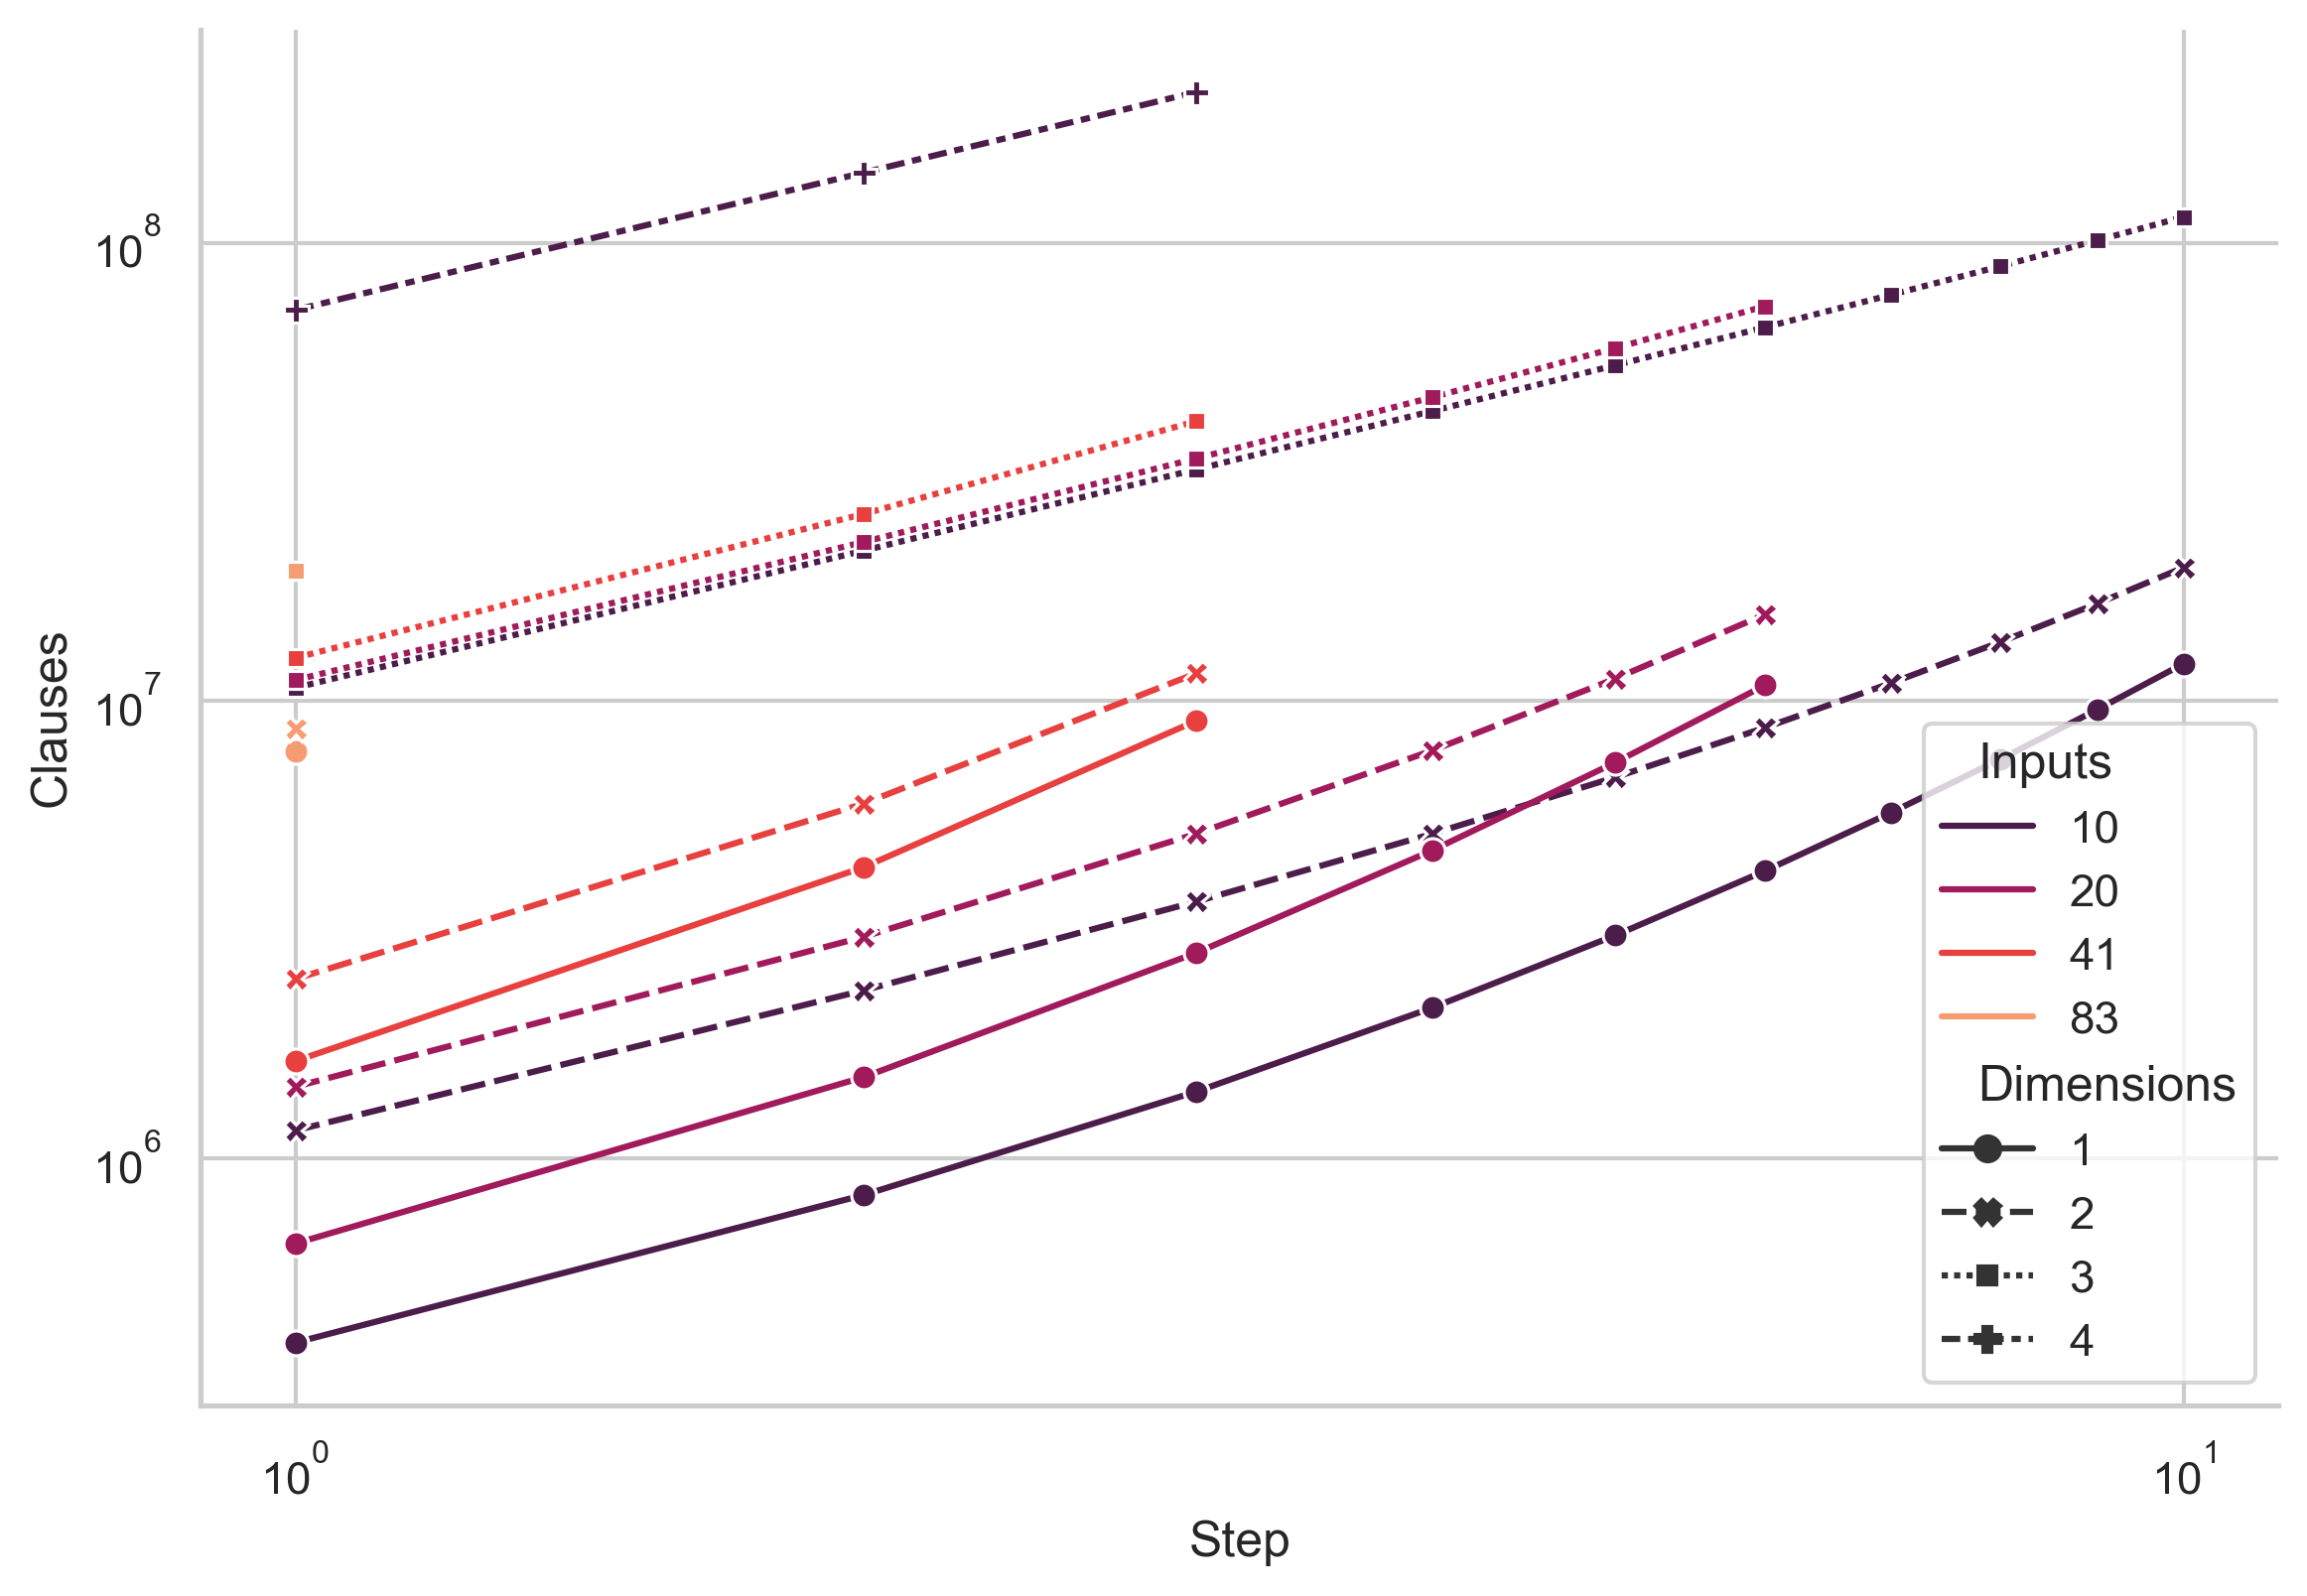
\includegraphics[width=\textwidth]{Tex//images/complexity_left.png}
        \caption{Number of Instantiated Clauses over Various Combinations of Workflow Length, Number of Inputs, and Dimensions.}
        \label{fig:native_ape_complex_left}
    \end{subfigure}%
    \hfill
    \begin{subfigure}[t]{.28\textwidth}
        \centering
        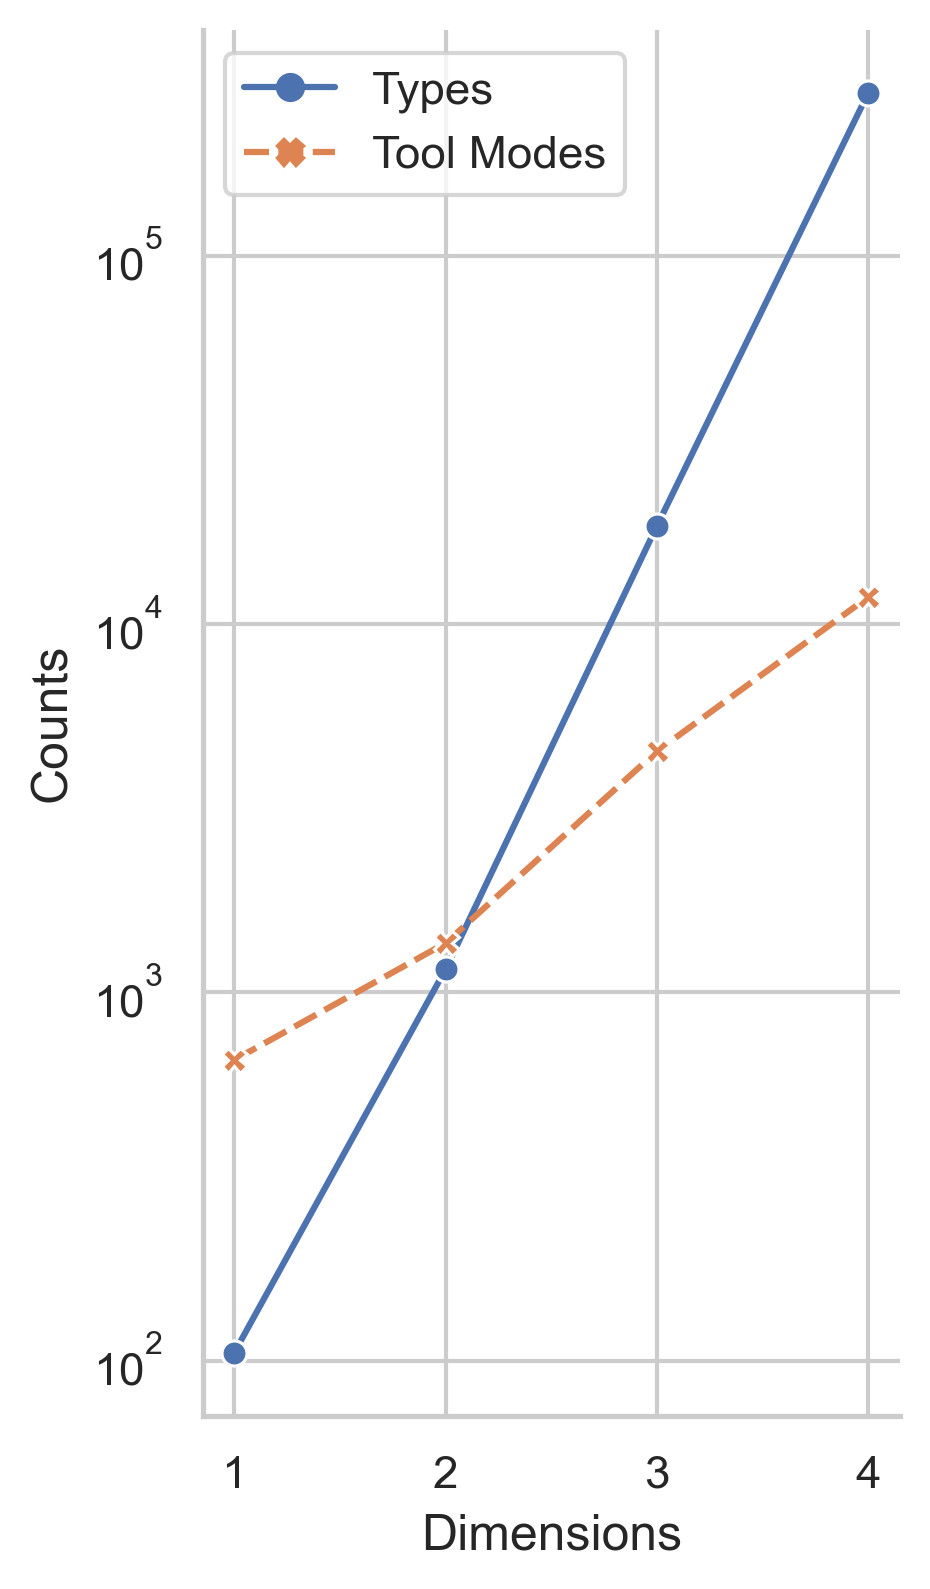
\includegraphics[width=\textwidth]{Tex//images/complexity_right.png}
        \caption{Tool and Type Taxonomy Sizes vs. Number of Type Dimensions.}
        \label{fig:native_ape_complex_right}
    \end{subfigure}
    \caption{Measurements from Search Complexity Experiments.}
    \label{fig:native_ape_double_complexity}
\end{figure}

The graph \autoref{fig:native_ape_complex_left} shows the seemingly linear relationship between the number of generated clauses and the workflow length. Interestingly, all experiments run out of heap space except for the configurations with three dimensions and ten inputs, and all runs with four dimensions, which timed out first.\footnote{The experiments were run on an Apple M1 Max with 8GB of assigned Java heap space. The timeouts on the runs with ten inputs occurred after roughly three and nine hours. The others did not finish setup for step one within more than double the given time limit and had to be interrupted externally. Run times longer than the stated 10000s might have been possible due to potentially missing timeout checks in the solver itself.} From this, we can infer that the memory usage of APE and its solver scale with more than just the number of clauses. Another observation is the significantly increasing complexity with rising input or dimension counts. The first relation is at least linear, while the second seems exponential, which is troubling since two dimensions already seem to limit the workflow length to eight, and using all four of them seems to cause a timeout or out-of-memory error after just one step.

Looking back at \autoref{eqn:workflow_sat_enc} assists in explaining the linear and exponential relationships. The top-level conjunctions scale linearly with the workflow length and the fixed tool parameter counts. Similarly, the inner disjunctions on unary predicates scale linearly with the number of possible types. Only the disjunction on the binary bind predicate would exceed linear growth. This fact is, however, made insignificant for the relatively low workflow length by the much larger sizes of the tool and type taxonomies shown in \autoref{fig:native_ape_complex_right}. The graph also indicates their exponential relationship with the number of dimensions\footnote{Adding one dimension potentially adds multiple new subtypes to every existing type, thus increasing both the number of types and explicit transition rules exponentially.}, which carries over into the number of generated clauses.

\section{Ontology Adaptation}
Addressing the in-place tool and complexity challenges requires the modification of the data science ontology. This subsection examines the changes in both the tool and the type taxonomy.

\subsection{Tool Taxonomy}
First, we will overview the new modes added to the toolset, reflecting the in-place data flow and reducing the overall number of tools required for modeling workflows. Notable affected tool sub-taxonomies include:

\begin{itemize}
    \item \textbf{Plotting}: These functions are kept as in-place tools since no labels need to be passed through. Usually, the inputs contain a table and various column selectors to produce a new plot instance. However, there could be problems when further customizing a figure, e.g., setting the figure size or label orientation. Some plotting data types must also be included in the tool inputs in these cases.
    \item \textbf{Estimators}: The fitting and prediction tools also continue to operate in-place. The state change from non-fit to fit is essential for implicit tool ordering. And even though model outputs could benefit from labels and data types, changing the tool to operate in-place would overwrite the original data.
    \item \textbf{Type casting}: Commonly, type casting would be done in-place, but the workflow constructed by APE would not be able to reflect the change in the type state. Hence, a non-in-place version is chosen that will lose the label but assign the correct type.
    \item \textbf{Data Splitting}: Both the non-in-place and the in-place versions are kept. However, neither can pass on a label to the new series split from the input table. The same happens when train-test-splitting: The non-in-place tool produces two new tables and two new series with no APE\_label values. Thus, controlling the data flow with these tools might only be possible when applying them last or defining the tool sequence directly via constraints.
    \item \textbf{Tabular Data Manipulation}: Most tools of this category have two versions to produce a copy of the data with no label or keep the label and modify the data in-place. Both options are standard in typical data science workflow.
    \item \textbf{Constructors}: Nontrained models are part of the input for training, tuning, or ensembling. To avoid hardcoding their instantiation into these tools and, thus, further enlarging the tool taxonomy, constructors for these estimators are added to the toolset. Their inputs are either empty or contain a string variable to allow the user to pass on a list of estimators.

    Another set of data types that need constructors is Matplotlib figures and axes. While most modifications are made after the tool produces the plot, setting the size and layout occurs during the figure and axis instantiation.
\end{itemize}

\subsection{Type Taxonomy}
Next, we will discuss the changes in the ontology's type taxonomy to reduce the search complexity. As shown in \autoref{fig:native_ape_double_complexity}, the number of clauses is influenced by multiple factors: the workflow length, number of inputs, and number of type dimensions. Even in its most minor configuration, APE ran out of heap space after ten steps. For this reason, data science applications will have to be split into multiple independent sections, and the notebooks will be joined outside of APE. The number of inputs is outside the scope of APE and entirely depends on which data importance assumptions the user has already made before synthesizing the workflow. However, as was shown, it is possible to use many inputs to create short tool sequences to help make these assumptions and filter the data for the actual workflow.

Lastly, we will give a brief rundown of the changes concerning the type taxonomies' dimensions:
\begin{itemize}
    \item The \verb|DataClass| dimension is the primary data type and is vital for differentiating type states. It is comparable to the data type of the objects in the Python backend. Hence, the dimension is kept in the taxonomy.
    \item \verb|StatisticalRelevance| is mainly for user convenience and clear separation of independent and dependent variables. The workflow might run without the dimensions, but the result could be misleading or incorrect. The dimension stays part of the ontology to avoid data leakage.
    \item The last two dimensions, \verb|DataState| and \verb|DataSetIndex|, are relevant for the executability of the workflow but add only little semantic value. Hence, they will be removed to reduce the complexity and allow workflow lengths of up to eight steps.
\end{itemize}

These changes to the ontology compromise the semantic quality of the synthesized workflows and their executability. They solve some of the challenges mentioned previously but also raise new concerns, mainly how tools with no output or no visible change in their parameter types influence the supposedly linear tool sequences produced by APE.

\section{Auxiliary Tools}
At this point, APE is able to produce tool sequences representing valid data science workflows. However, some auxiliary tools are still required to enable an automated workflow. The following subsections will introduce four new steps or tools in the APE workflow for data science.

\subsection{Input Data Preparation}
The tool is implemented as a Python script designed to load input data consistent with how it will be read in the subsequent APE-generated workflow. Upon reading the data frames, the tool detects the data type of each column and assigns a corresponding type state. The read feature labels are used as values for the \verb|APE_label| dimension. By passing a list of dependent variables for each table to the tool, users enable it to annotate the columns' type states in the \verb|StatisticalRelevance| dimension. If desired, the tool can split the table into separate data frames, each containing dependent or independent variable columns, and create respective type states for them.

\begin{table}[h]
\centering
\begin{tabular}{|c|c|c|c|c|}
\hline
PassengerID & Name & Sex & Age & Survived \\
\hline
int64 & str & str & int64 & int64 \\
\hline\hline
... & ... & ... & ... & ... \\
\hline
\end{tabular}
\caption{Sample Schema Excerpt from the Titanic Data Set.}
\label{table:native_ape_data_prep_sample_table}
\end{table}

The sample \autoref{table:native_ape_data_prep_sample_table} has three integer and two string-type columns and is annotated with its Numpy data types. Additionally, all columns are independent except for Survived. First, the tool matches these with their \verb|DataClass| dimension counterparts and annotates the type states accordingly. Even though each column is identified by a string, the \verb|APE_label| value, and is processed as such in the workflow to notebook transformation, the ontology has a specific sub-taxonomy to mark data series that are part of a table to handle table-column associations. The input configuration, representing the table in APE, is shown in \autoref{code:native_ape_data_prep_config} and contains another entry for the table in addition to the five columns.
\begin{lstlisting}[language=json, caption=Input Config for Sample Table., label=code:native_ape_data_prep_config]
"inputs": [
  {
    "DataClass": ["IntColumn"],
    "StatisticalRelevance": ["IndependentVariable"],
    "APE_label": ["PassengerID"]
  }, {
    ...
  }, {
    "DataClass": ["IntColumn"],
    "StatisticalRelevance": ["DependentVariable"],
    "APE_label": ["Survived"]
  }, {
    "DataClass": ["MixedDataFrame"],
    "StatisticalRelevance": ["None"],
    "APE_label": ["titanic_train"]
  }
]
\end{lstlisting}

\subsection{Output Parser}
After APE finishes synthesizing valid tool sequences, additional tools are required to transform these into executable programs. Internally, APE represents each found solution with a graph encoded as a set of tool-, type-, and bind-predicates \cite{kasalica2022synthesis}. Notably, all these graphs are stored in a single solution file. The output parsing process loads this file and transforms each of the contained declarative workflow definitions into a linear sequence of tools and their input parameter dependencies. A crucial part of this step is the extraction of the terminal tool and type predicates from among all their parent taxonomy terms produced by APE's encodings, followed by the reconstruction of type states. The latter is done by collecting and grouping the dimension values for each step and parameter index.

In specific scenarios, APE introduces a new plain type to ensure that all concrete data types are leaves within the type taxonomy. This must be accounted for when constructing the script with actual Python object types. Finally, the intermediary workflow format, and the last artifact before the notebook construction, is a JSON file containing the solution’s inputs, outputs, and tool sequence. Each step object includes its tool, parameter type states, and which previous tool output each of its inputs is bound to, as shown in \autoref{code:native_ape_output_parsing}.

\begin{lstlisting}[language=json, caption=Step in JSON Workflow Encoding., label=code:native_ape_output_parsing]
{
  "tool": "lineplot_12",
  "input": [
    {
      "DataClass": "IntSeries",
      "StatisticalRelevance": "IndependentVariable",
      "APE_label": ["Pclass"],
      "src": [0, 2]
    },
    ...
  ],
  "output": [
    {
      "DataClass": "Axes",
      "StatisticalRelevance": "NoRelevance"
    }
  ]
}
\end{lstlisting}

\subsection{Python Tool Library}
The tools in the data science ontology and their modes are implemented with Python and can be imported from this module. Each function implements exactly one tool, and multiple modes are represented by overloading the function signatures and adding the required branches to the function. The implementations bundle common function call sequences to simplify the interpretation and extension of the workflow notebooks, such that each step in the notebook is reduced to one line of code. Furthermore, they also include methods to display outputs and intermediary results, primarily tables, plots, and numeric statistics, where deemed sensible. While not necessarily part of the final workflow output, these tool outputs may interest the user and would otherwise disappear since they are immediately assigned to variables in the notebook.

In addition to the main libraries, which split the tools at the top level, the following libraries provide further functionality in the implementations:
\begin{itemize}
    \item \textbf{Pandas} and \textbf{Numpy} to store and transform tabular data.
    \item \textbf{Scipy} for computing and checking statistical assumptions.
    \item \textbf{scikit-learn} for simple modeling.
    \item \textbf{Matplotlib} and \textbf{Seaborn} for creating graphs.
    \item \textbf{Gensim}, \textbf{Wordcloud}, \textbf{Spacy}, \textbf{BS4}, and \textbf{Textblob} for text analysis.
\end{itemize}

The function names and signatures are kept close to their source library equivalent to simplify extending and adapting the result for users that already have Python data science skills. Many tools are simplified by default. Optional keyword arguments allow the user to pass in more parameters outside of the APE workflow and, thus, will enable the customization of the results without increasing the synthesis complexity.

\subsection{Executable Notebook Construction}
After parsing them into a JSON file, each of the found solutions is finally transformed into a Jupyter Notebook. It provides the required framework to execute the script and displays the underlying code, markdown texts, LaTeX snippets, and images.

\paragraph{Header}
At the top of each notebook, the solution's graph generated by APE is displayed for a general workflow overview. The necessary imports, such as the tool module and input loading libraries, follow this.

\paragraph{Inputs}
The next segment of the notebook, shown in \autoref{fig:native_ape_nb_inputs}, focuses on the workflow inputs. Each input is isolated in its own cell and annotated with its corresponding data state, identifier, and source in markdown. The symbol names are chosen by the user and defined during the data preparation.

\begin{figure}
    \centering
    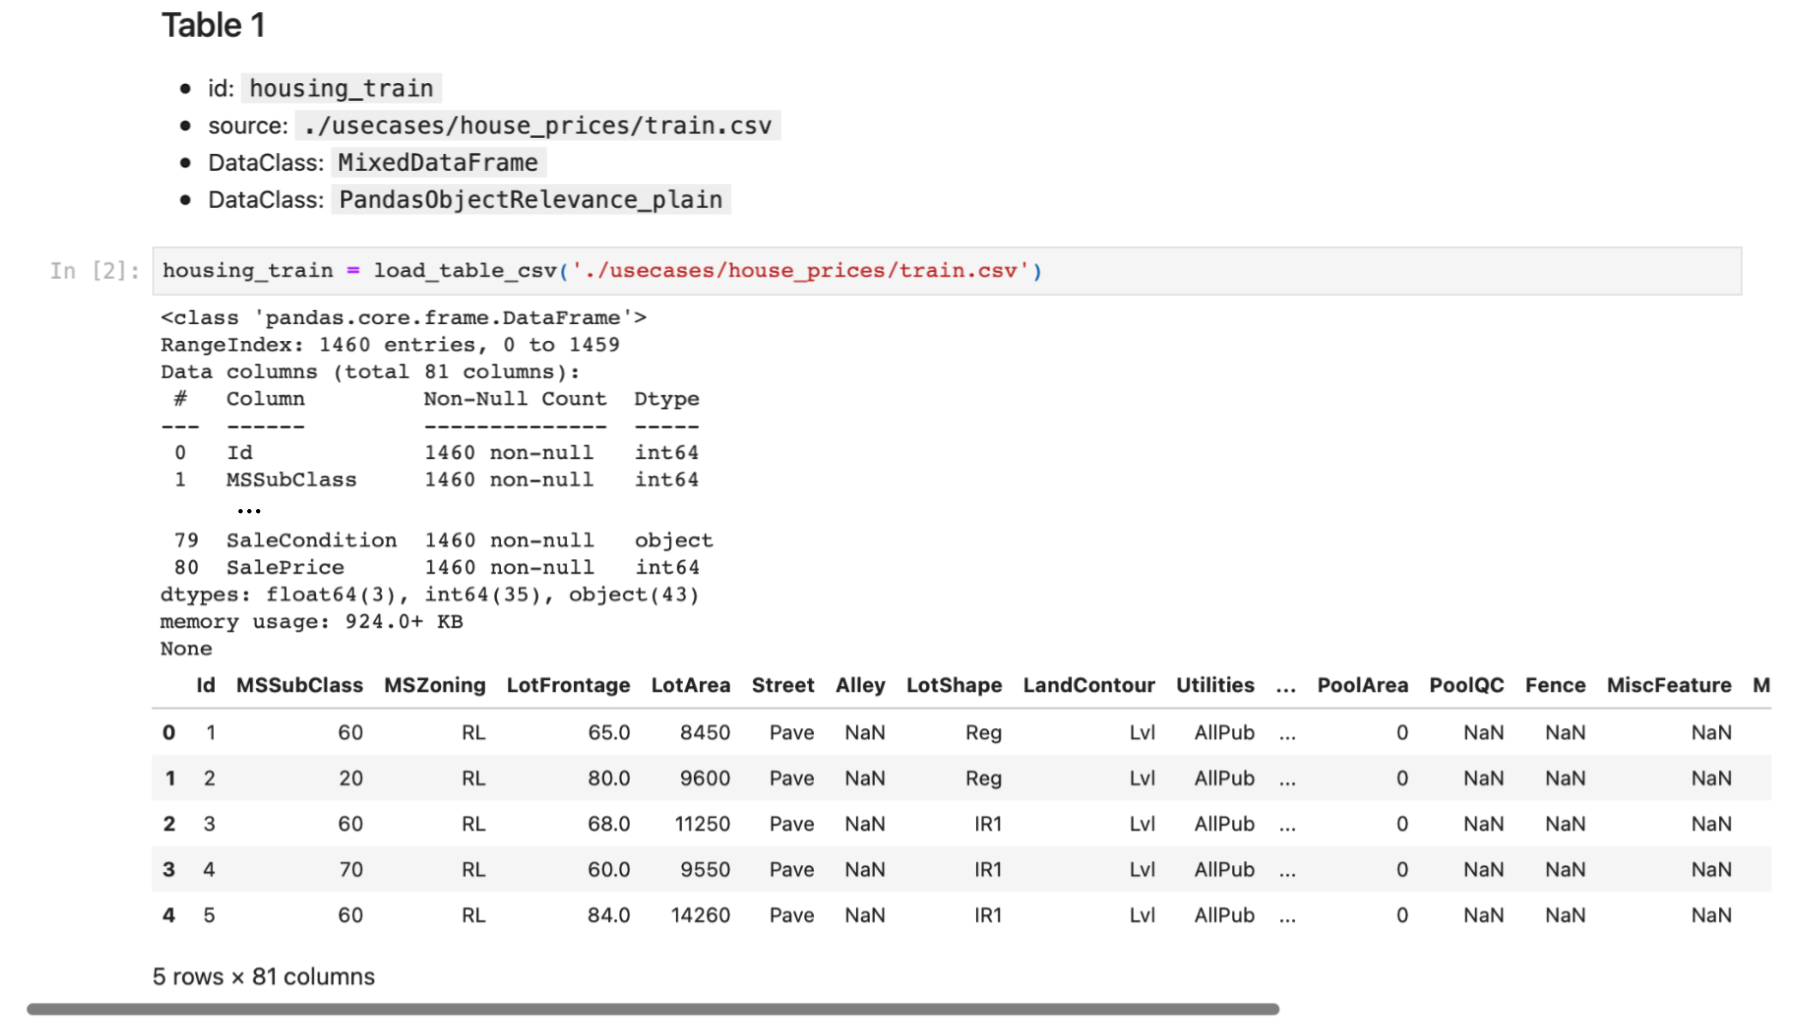
\includegraphics[width=\textwidth]{Tex/images/native_ape_nb_inputs.png}
    \caption{Workflow Inputs Section in Jupyter Notebook.}
    \label{fig:native_ape_nb_inputs}
\end{figure}

\paragraph{Tool Sequence}
Subsequently, the workflow steps are listed in the notebook’s primary section. Each step is structured to include a title with its step number and tool name, the type states for inputs and outputs, the dependency of each input parameter, the docstring for the tool being used, and finally, the function call, see \autoref{fig:native_ape_nb_step}.

\begin{figure}
    \centering
    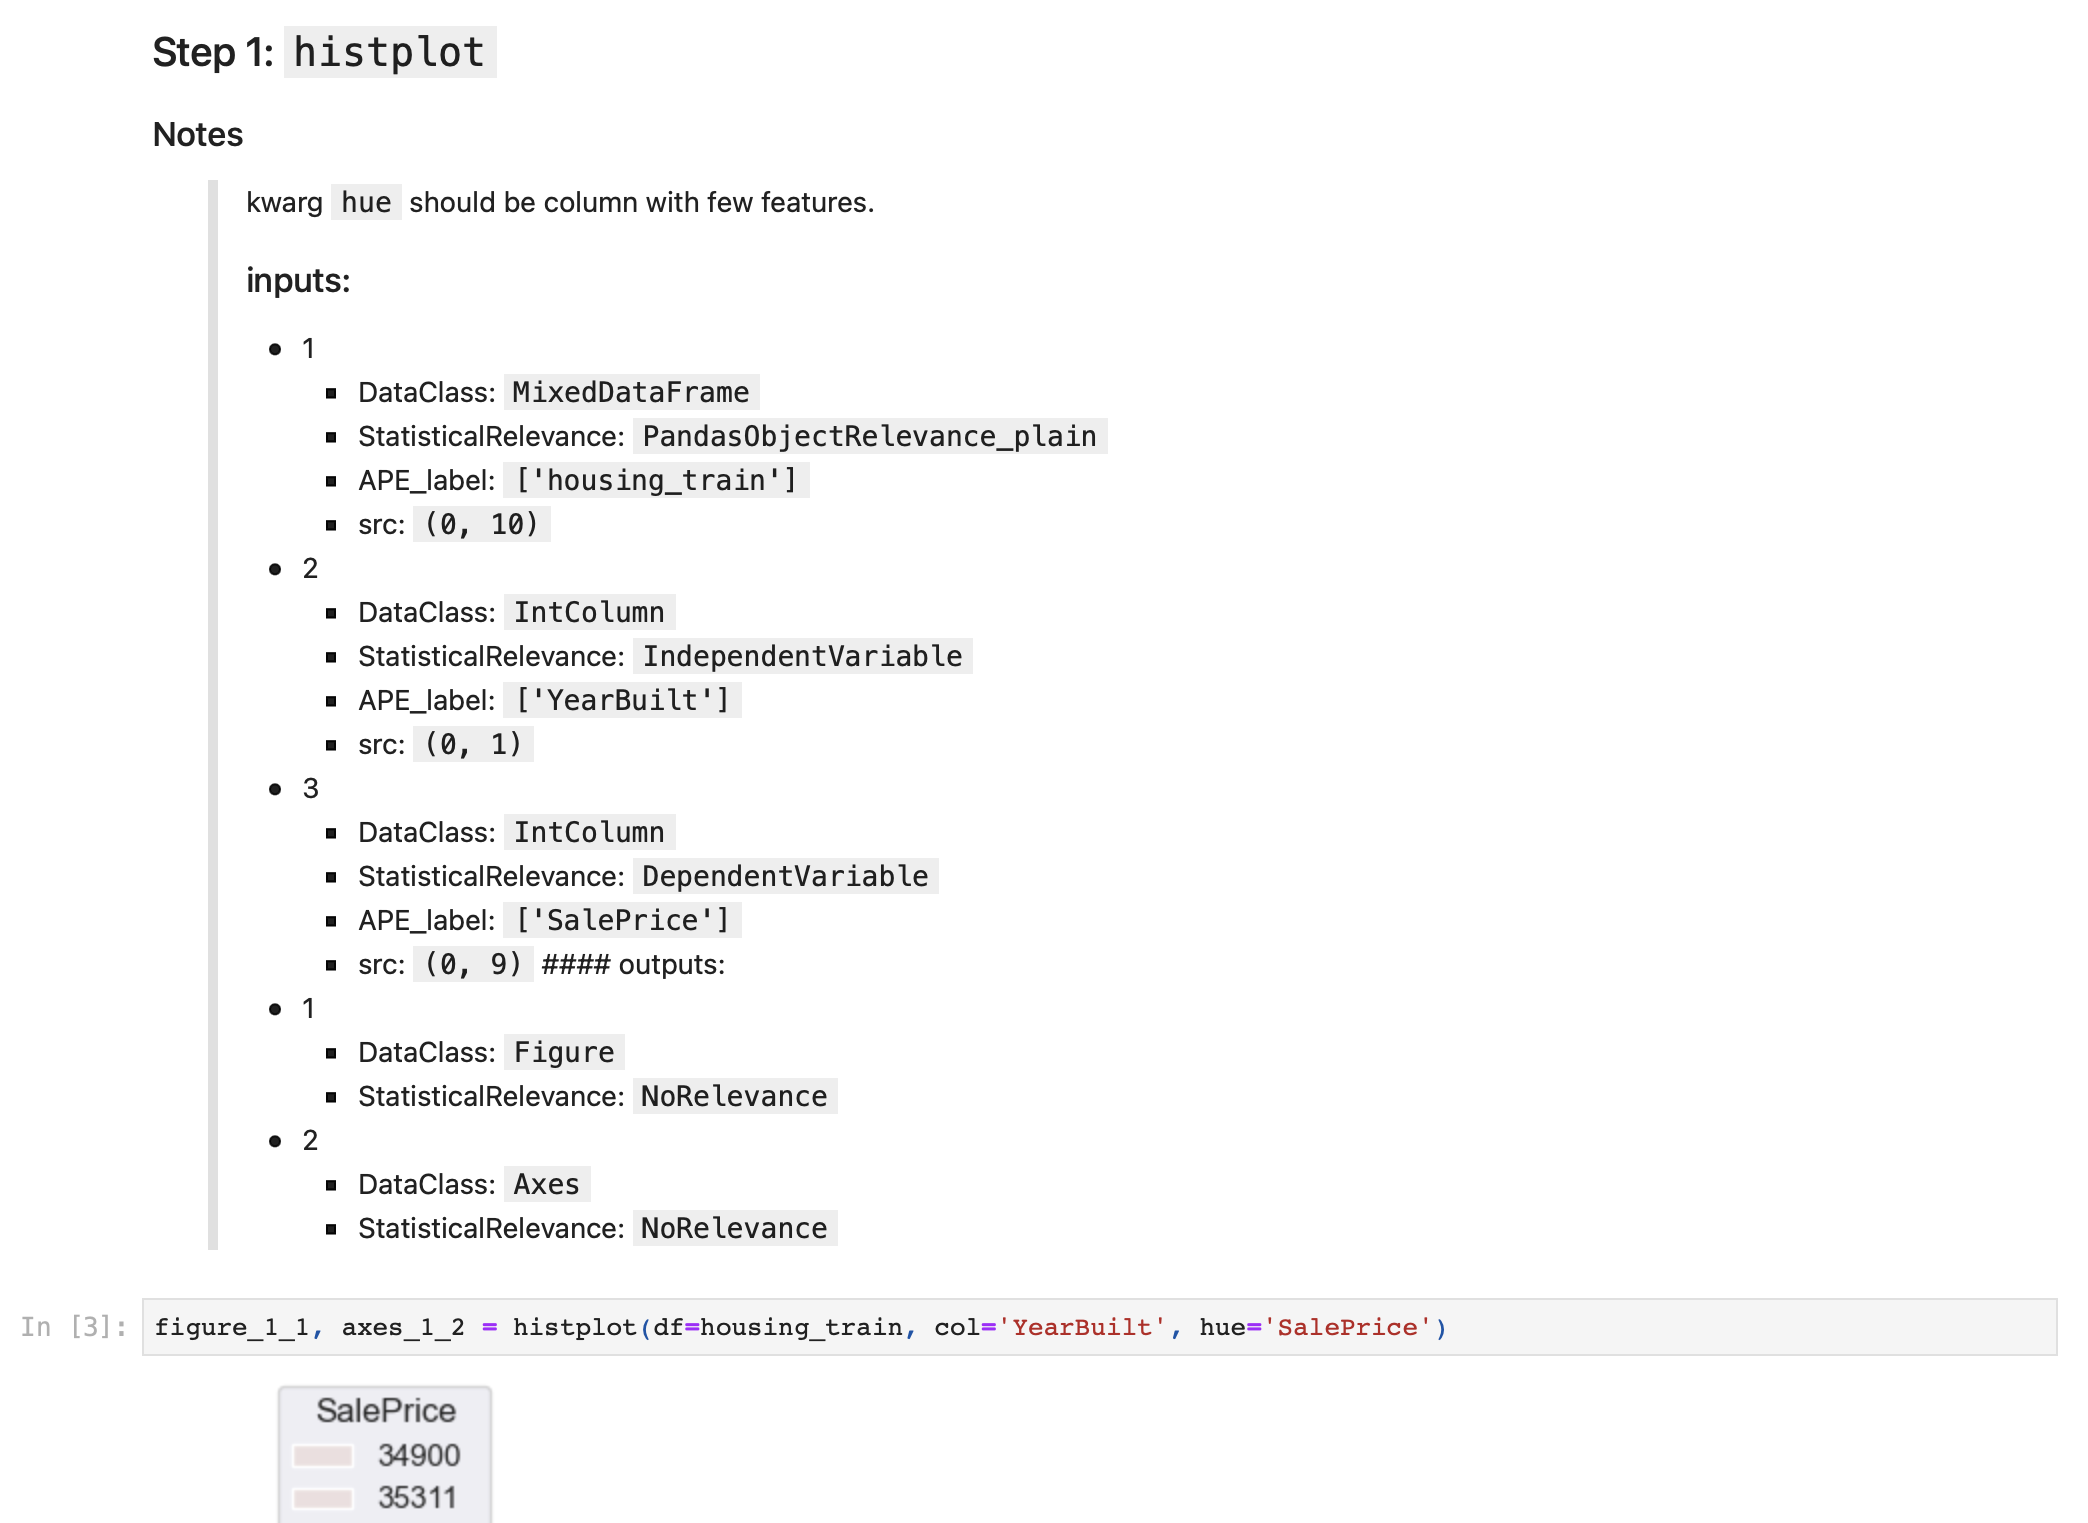
\includegraphics[width=\textwidth]{Tex/images/native_ape_nb_step.png}
    \caption{Step Description, Code Cell, and Part of the Graph Output.}
    \label{fig:native_ape_nb_step}
\end{figure}

The Python tool docstrings are listed under \verb|Notes| and may elaborate on its functionality and arguments or include warnings about its usage. This is especially beneficial when the parameters APE assigned may not match the implementation's semantic requirements, such as in the following scenarios.
\begin{itemize}
    \item \textbf{Plotting}: The \verb|hue| or \verb|style| parameter may hold the label of a column with arbitrary type. However, too many unique values in that column, like in the case of a numeric identifier feature, might render the result less meaningful. For this reason, the example in \autoref{fig:native_ape_nb_step} includes a warning concerning the hue parameter usage. There, the affected argument is matched with the \verb|SalePrice| column of type float.
    \item \textbf{User-defined values}: Labels may be introduced in the input config. Since these potentially new types can not be checked in the tool transitions, they are passed directly through the notebooks and Python tools. The advantage of this is the simplification of the taxonomy while still allowing complex inputs. The disadvantage is that the unchecked input may be syntactically wrong or make no sense in the context.
\end{itemize}

A Python code cell contains the function call with its output assignment. The identifiers for these new variables consist of the data class, step number, and output parameter index for more straightforward interpretability. Input parameters are passed to the function with keyword arguments to remove any ambiguity. However, overloaded tools complicate pairing the type states to their correct Python keyword argument. Specifically, we can not differentiate multiple identical type states; thus, the first matching parameter is assigned by default. For example, plotting functions may use the optional parameters \verb|hue| and \verb|style| to adjust the look of the plot. However, both expect the same data type: It is unclear which keyword the third parameter in \autoref{fig:native_ape_nb_step} is meant for. Since \verb|hue| is listed before \verb|style| in the function signatures, it is currently impossible to automatically assign the latter without assigning the first. Basic object and column type states, such as inputs 2 and 3, are passed to the function directly. In contrast, other complex types are passed as references to their previously created variables.

\paragraph{Outputs}
The final section of the notebook displays the workflow outputs. Similarly to the inputs and tool step sections, this includes their type states, the tool responsible for generating them, and their respective output indices.

\section{Alternative ASP Backend}\label{sec:asp_backend}

As used in this project, APE uses an off-the-shelf SAT solver \cite{kasalica2022synthesis} to search for valid workflows, and the domain ontology and constraints are translated from more practical formats, such as Owl or JSON. The only other way to interact with the synthesis process is the composition of custom constraints using SLTLx. However, since even this expressive language is encoded into the SAT instance, many of the related challenges regarding user interaction remain. This section will introduce an alternative solver backend for the APE synthesis concept using ASP.

\subsection{APE Encodings}
The domain and workflow encoding are directly translated versions of their SAT counterparts. Where necessary, the predicates are split into multiple rules and constraints. \autoref{code:asp_back_workflow_enc} shows the set of ASP rules encoding the workflow from \autoref{eqn:workflow_sat_enc}. Specifically, this snippet represents the top-level generation of predicates with choice rules that will be filtered by the constraints. Similar to APE increasing the workflow length by one each time the solver does not find sufficient solutions, the ASP backend uses incremental solving with Python to iteratively instantiate and search. Here, for each new step \verb|t|, the instance is extended by choices for the used tool, parameters, and data bindings: Lines 2 and 3 ensure that at least one tool is used during the step. Lines 4 through 11 assign at least one type to each parameter position and dimension. Finally, lines 12 through 23 connect non-empty tool inputs to previously generated outputs from steps \verb|0| to \verb|t-1| for each input index, with the workflow output being encoded as the input of step \verb|-1|. The empty type \verb|eps| is the only value of the \verb|null| dimensions and ensures exclusivity to other dimensions.

\resetJsonFlag
\begin{lstlisting}[language=Prolog, caption=SAT Workflow Predicate Encoded as ASP Rules., label=code:asp_back_workflow_enc, numbers=left,numberstyle=\tiny]
% [[W]]_n 
1 = { use_tool(Tool, t) : term_tool(Tool) }.
1 { use_tool(Tool, t) : tool(Tool) }.
1 {
    in((t, Ix), Dim, Type) : type(Dim, Type)
} :- Ix=1..MaxIn,
     tool_input_ix_max(MaxIn).
1 {
    out((t, Ix), Dim, Type) : type(Dim, Type)
} :- Ix=1..MaxOut,
     tool_output_ix_max(MaxOut).
1 {
    bind((t, IxIn), (0..t-1, 1..MaxOut))
} :- IxIn=1..MaxIn,
     tool_input_ix_max(MaxIn),
     tool_output_ix_max(MaxOut),
     not in((t, IxIn), null, eps).
{
    bind((-1, IxIn), (t, 1..MaxOut))
} :- IxIn=1..MaxIn,
     tool_input_ix_max(MaxIn),
     tool_output_ix_max(MaxOut),
     not in((-1, IxIn), null, eps).
\end{lstlisting}

\subsection{APE Extensions}
Deploying an ASP backend instead of SAT provides the user with several new ways of interacting with the solver. The most notable are heuristics and soft constraints. Both enable the user to introduce domain and workflow knowledge in the form of preferences for the aforementioned choice rules. These constructs, exemplified in lines 1 through 8 of \autoref{code:asp_back_heuristics}, change the search order to, e.g., favor plotting tools over modeling tools during the solving process or reduce the chances of an input appearing twice in a step. These preferences could improve the quality of the found results by ordering the vast amount of types and tool modes originating from general-purpose libraries. Moreover, in addition to natural language templates and SLTLx formulas, constraints could be encoded into the ontology directly while still being interpretable. For example, lines 10 through 15 show a hard constraint limiting visualization steps binding of \verb|Figure| and \verb|Axes| inputs to the same source step to ensure tool executability.

\begin{lstlisting}[language=Prolog, caption=ASP Heuristics Encoding Domain and User Preferences., label=code:asp_back_heuristics, numbers=left,numberstyle=\tiny]
% Usually no modeling
#heuristic in((t _),"DataClass","SklearnObject").
           [40,false]
#heuristic use_tool(t,"Modeling"). [40,false]
% Avoid using the same input twice
#heuristic in((t,X),"APE_label",COL):
           in((t,Y),"APE_label",COL),
           X != Y. [10,false]

% Use same source for figure and axes inputs
:- in((t,IxF),"DataClass","Figure"),
   in((t,IxA),"DataClass","Axes"),
   bind((t,IxA),(T1,_)),
   bind((t,IxF),(T2,_)),
   T1 != T2.
\end{lstlisting}

\subsection{Future Work}
While this alternative backend might improve on some usability aspects of APE, it also introduces longer solving times on larger workflow problems. The computational overhead from directly translated SAT encodings could be reduced by rewriting the rules from the ground up following ASP best practices. Notably, the most significant modification would be compromising on the general purpose ontology compatibility and tailoring the backend to the data science domain. As a result, the framework could include ASP rules for tool annotations with real generics and passthrough parameters, nested types, and weight optimization - mostly ASP native features.
